\section{Spracherweiterungen}
In diesem Abschnitt werden die geplanten Erweiterungen an der Sprache erläutert. 
Ein wichtiges Kriterium für unsere Erweiterungen war es, die Kompatibliität von 
zur Standard-IML beizubehalten. Es muss möglich sein, bereits vorhandene Programme
auch mit dem erweiterten Compiler zu kompilieren und eine äquivalentes Programm zu 
erhalten. Dies macht es zudem leichter, bestehende IML Programme um pre-/postconditions
zu erweitern. In den folgenden Abschnitten wird festgehalten, in welchem Ausmass dies 
gelingen kann. Die Änderungen an der Grammatik sind in Anhang \ref{sec:grammar} dokumentiert.

\subsection{Pre-/Postconditions}
Das definieren von pre- und postconditions sollte direkt beim Deklarieren
der Prozedur oder der Funktion ermöglicht werden. So sind die Garantien
für den Programmierer auf einen Blick ersichtlich und erleichern so 
das Verständnis der Prozedur. In Listing \ref{lst:first} ist ein Beispiel 
einer Prozedur mit conditions ersichtlich.


\begin{lstlisting}[caption=Beispiele von pre-/postconditions,label={lst:first}]
proc divide(in copy m:int32, in copy n:int32, out ref q:int, out ref r:int32)
requires [n > 0, unnecessary(m, n)]
ensures [r >= 0]
{
    q init := 0;
    r init := m;

    while(r >= n) {
        q := q+1;
        r := r-n;
    }
}
\end{lstlisting}


\subsection{Zugriff auf pre-execution state}

Der Zugriff auf die Werte der Variablen vor der Ausführung der Prozedur ist 
von entscheidender Bedeutung für das Definieren von post conditions. Nur so 
kann beispielsweise überprüft werden, dass sich das Vorzeichen einer Variable
nicht geändert hat, oder das ein neuer Wert einer Variable im Vergleich zum 
Alten grösser geworden ist. Dies verlangt nach einem Konstrukt, welches 
es dem Programmierer erlaubt festzulegen, ob auf den Wert der Variablen
nach der Ausführung oder vor der Ausführung der Prozedur zugegriffen werden kann.

Wir haben uns für das Definieren einer reservierten Funktion namens \textit{old} 
entschieden. Dies hat den Vorteil, dass die Grammatik nicht komplexer wird. Jedoch 
muss ein neuer Kontext-Check eingeführt werden, welcher überprüft, dass kein Namenskonflikt
mit einer existierenden Funktion auftritt. Zudem muss überprüft werden, ob \textit{old} 
nur innerhalb von postconditions auftritt.

\begin{lstlisting}[caption=Beispiel eines Zugriffs auf alten Zustand,label={lst:old_state}]
proc divide(in copy m:int32, in copy n:int32, out ref q:int, out ref r:int32)
ensures [old(n) > r]
{
    q init := 0;
    r init := m;

    while(r >= n) {
        q := q+1;
        r := r-n;
    }
}
\end{lstlisting}


Siehe Anhang \ref{sec:Grammar}

%\newpage

%\begin{figure*}[h]
%	\begin{center}
%		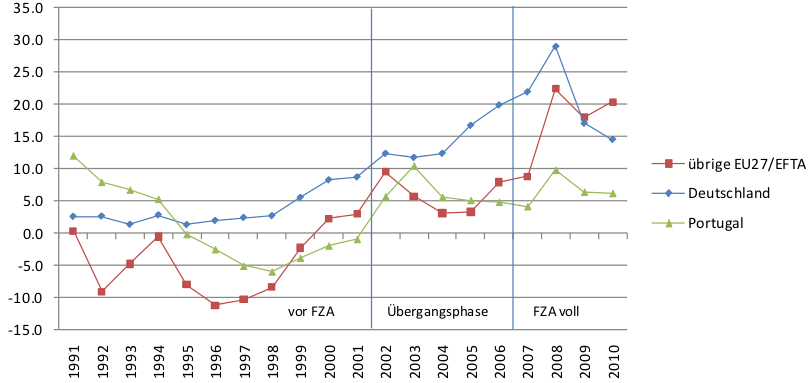
\includegraphics[width=0.9\textwidth]{images/Zuwanderungssaldo_Bericht_2.png}
%	\end{center}
%	\caption{Verlauf der Zuwanderung nach Herkunftsländern in Tausend \cite[S. 18]{ADMIN:Bericht}}
%	\label{fig:zuwanderungsaldi}
%\end{figure*}

